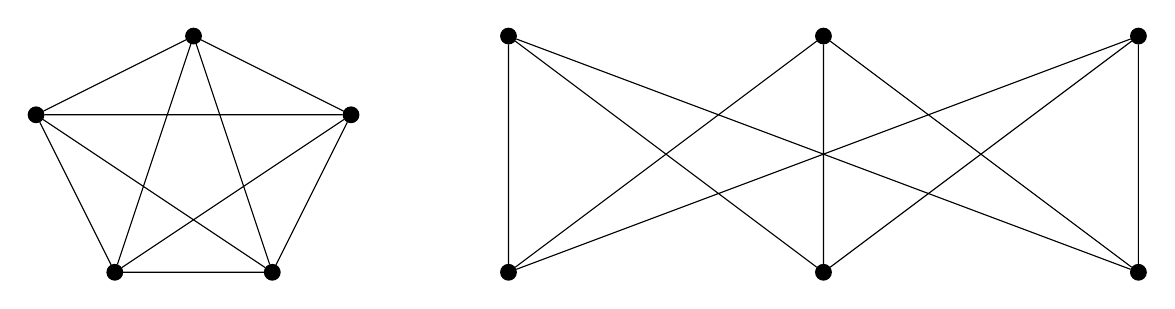
\begin{tikzpicture}[every node/.style={draw,inner sep=2pt,fill=black}]
      \path[shape=circle]
	(2,3) node(a1){} (6,0) node(x1){} (10,0) node(x2){} (14,0) node(x3){} 
	(0,2) node(b1){} (4,2) node(b2){}
	(1,0) node(c1){} (3,0) node(c2){}  (6,3) node(y1){} (10,3) node(y2){} (14,3) node(y3){};
	\filldraw (a1) -- (b1) -- (c1) -- (c2) -- (b2) -- (a1) -- (c1) -- (b2) -- (b1) -- (c2) -- (a1);
	\filldraw (x1) -- (y1) -- (x2) -- (y2) -- (x3) -- (y3) -- (x1) -- (y2);
	\filldraw (x2) -- (y3);
	\filldraw (y1) -- (x3);
\end{tikzpicture}